% Options for packages loaded elsewhere
\PassOptionsToPackage{unicode}{hyperref}
\PassOptionsToPackage{hyphens}{url}
%
\documentclass[
]{book}
\usepackage{lmodern}
\usepackage{amssymb,amsmath}
\usepackage{ifxetex,ifluatex}
\ifnum 0\ifxetex 1\fi\ifluatex 1\fi=0 % if pdftex
  \usepackage[T1]{fontenc}
  \usepackage[utf8]{inputenc}
  \usepackage{textcomp} % provide euro and other symbols
\else % if luatex or xetex
  \usepackage{unicode-math}
  \defaultfontfeatures{Scale=MatchLowercase}
  \defaultfontfeatures[\rmfamily]{Ligatures=TeX,Scale=1}
\fi
% Use upquote if available, for straight quotes in verbatim environments
\IfFileExists{upquote.sty}{\usepackage{upquote}}{}
\IfFileExists{microtype.sty}{% use microtype if available
  \usepackage[]{microtype}
  \UseMicrotypeSet[protrusion]{basicmath} % disable protrusion for tt fonts
}{}
\makeatletter
\@ifundefined{KOMAClassName}{% if non-KOMA class
  \IfFileExists{parskip.sty}{%
    \usepackage{parskip}
  }{% else
    \setlength{\parindent}{0pt}
    \setlength{\parskip}{6pt plus 2pt minus 1pt}}
}{% if KOMA class
  \KOMAoptions{parskip=half}}
\makeatother
\usepackage{xcolor}
\IfFileExists{xurl.sty}{\usepackage{xurl}}{} % add URL line breaks if available
\IfFileExists{bookmark.sty}{\usepackage{bookmark}}{\usepackage{hyperref}}
\hypersetup{
  pdftitle={MBL617 Theory and Methods in Digital Heritage},
  pdfauthor={Özgün Balaban Güzden Varinlioğlu},
  hidelinks,
  pdfcreator={LaTeX via pandoc}}
\urlstyle{same} % disable monospaced font for URLs
\usepackage{longtable,booktabs}
% Correct order of tables after \paragraph or \subparagraph
\usepackage{etoolbox}
\makeatletter
\patchcmd\longtable{\par}{\if@noskipsec\mbox{}\fi\par}{}{}
\makeatother
% Allow footnotes in longtable head/foot
\IfFileExists{footnotehyper.sty}{\usepackage{footnotehyper}}{\usepackage{footnote}}
\makesavenoteenv{longtable}
\usepackage{graphicx,grffile}
\makeatletter
\def\maxwidth{\ifdim\Gin@nat@width>\linewidth\linewidth\else\Gin@nat@width\fi}
\def\maxheight{\ifdim\Gin@nat@height>\textheight\textheight\else\Gin@nat@height\fi}
\makeatother
% Scale images if necessary, so that they will not overflow the page
% margins by default, and it is still possible to overwrite the defaults
% using explicit options in \includegraphics[width, height, ...]{}
\setkeys{Gin}{width=\maxwidth,height=\maxheight,keepaspectratio}
% Set default figure placement to htbp
\makeatletter
\def\fps@figure{htbp}
\makeatother
\setlength{\emergencystretch}{3em} % prevent overfull lines
\providecommand{\tightlist}{%
  \setlength{\itemsep}{0pt}\setlength{\parskip}{0pt}}
\setcounter{secnumdepth}{5}
\usepackage{booktabs}
\usepackage{amsthm}
\makeatletter
\def\thm@space@setup{%
  \thm@preskip=8pt plus 2pt minus 4pt
  \thm@postskip=\thm@preskip
}
\makeatother
\usepackage[]{natbib}
\bibliographystyle{apalike}

\title{MBL617 Theory and Methods in Digital Heritage}
\author{Özgün Balaban Güzden Varinlioğlu}
\date{}

\begin{document}
\maketitle

{
\setcounter{tocdepth}{1}
\tableofcontents
}
\hypertarget{intro}{%
\chapter{Syllabus}\label{intro}}

\hypertarget{content}{%
\section{Content}\label{content}}

The course is an introduction to \textbf{Digital Heritage} and has a two-fold purpose. In addition to giving an overview of theories and principles in digital heritage, both in Turkey and internationally, the course gives an introduction to research methods in three areas related to cultural heritage: \textbf{collection/management, visualization/communication,} and \textbf{analysis/ interpretation.}

\hypertarget{aims}{%
\section{Aims}\label{aims}}

To help students understand the link between cultural heritage and computing; to introduce key issues in digital heritage; to provide students with the basic theoretical and practical knowledge of digital methods such as GIS, AR/VR, AI.

\hypertarget{learning-outcomes}{%
\section{Learning outcomes}\label{learning-outcomes}}

Students who take this course gain will knowledge, ability and proficiency in the following subjects:

\begin{itemize}
\tightlist
\item
  Knowledge of historical, contemporary and specialized issues in the area of visual computation through original research,
\item
  Understanding of the interdisciplinarity of computation in cultural heritage,
\item
  Ability to assess methods and applications of digital heritage through systematic approaches,
\item
  Ability to assess and apply research methodology,
\item
  Competence in creative and critical thinking, problem-solving and decision making.
\end{itemize}

\hypertarget{conduct}{%
\section{Conduct}\label{conduct}}

The course will be conducted as seminars with weekly readings and assignments. During the course of the semester, students are required to submit written and practical assignments as requested by the instructors during class, and one final paper, based on either literature research or an original argument, and an in-class presentation of the final paper at the semester end. The essays submitted throughout the semester are to constitute the basis for the final paper; these should take into account class discussions, as well as students' own reflections. The final paper should be around 3000 words and structured with an introduction, development, and conclusion. The grading for the course is as follows: attendance and in-class participation in discussions and weekly response papers, 30\%; hands-on practices, 30\%; one end-of-semester paper, 20\%; final project presentation by individual/group 20\%.

\hypertarget{project}{%
\section{Project}\label{project}}

The collective efforts of the course participants will be part of a digital heritage project on Caravanserais of Anatolia. \textbf{All works will be uploaded to the website.}

\hypertarget{weekly-schedule}{%
\section{Weekly Schedule}\label{weekly-schedule}}

\hypertarget{quick-start-to-qgis}{%
\chapter{Quick Start to QGIS}\label{quick-start-to-qgis}}

\hypertarget{installing-qgis}{%
\section{Installing QGIS}\label{installing-qgis}}

There are two options for installation:\\
* OSGeo4\\
* Standalone Installer

\hypertarget{familiarizing-yourself-with-qgis-desktop}{%
\section{Familiarizing yourself with QGIS Desktop}\label{familiarizing-yourself-with-qgis-desktop}}

\begin{figure}
\centering
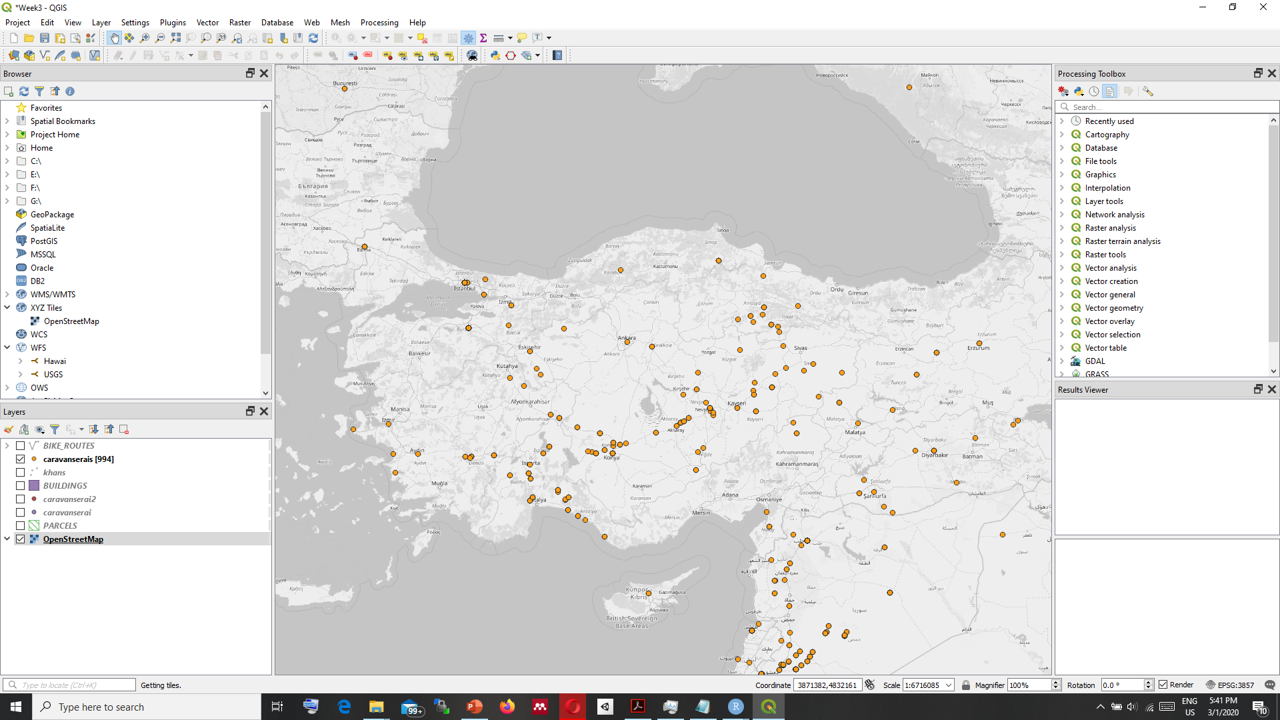
\includegraphics{Images/gui.png}
\caption{QGIS GUI}
\end{figure}

\begin{enumerate}
\def\labelenumi{\arabic{enumi}.}
\tightlist
\item
  Menu Bar
\item
  Toolbars
\item
  Panel
\item
  Map Canvas
\item
  Status Bar
\end{enumerate}

\hypertarget{vector-data}{%
\chapter{Vector Data}\label{vector-data}}

\hypertarget{types-of-vector-data-in-qgis}{%
\section{Types of vector data in QGIS}\label{types-of-vector-data-in-qgis}}

\begin{itemize}
\tightlist
\item
  Points
\item
  Lines
\item
  Polygons
\end{itemize}

\begin{quote}
layer \textgreater{} add layer \textgreater{} add vector layer
\end{quote}

\begin{figure}
\centering
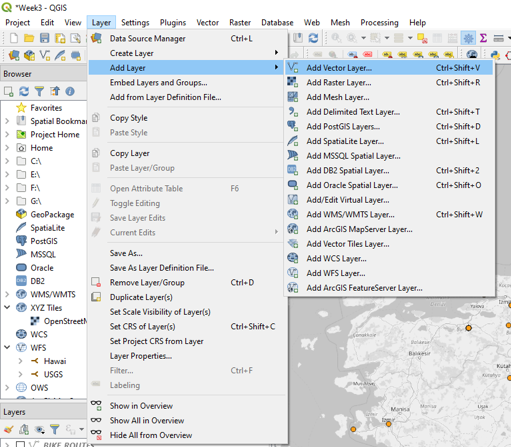
\includegraphics{Images/addVectorLayer.png}
\caption{Adding Vector Layer}
\end{figure}

\begin{itemize}
\tightlist
\item
  File
\item
  Folder
\item
  Database
\item
  Protocol
\end{itemize}

Files that can be loaded as vector files:

\begin{itemize}
\tightlist
\item
  Geopackage
\item
  ESRI Shapefile
\item
  Geography Markup Language
\item
  CSV
\item
  \ldots{}
\end{itemize}

WFS data example:
\url{https://mrdata.usgs.gov/services/wfs/ofr20051294?request=GetCapabilities\&service=WFS\&version=1.1.0}

\hypertarget{raster-data}{%
\chapter{Raster Data}\label{raster-data}}

\begin{itemize}
\tightlist
\item
  Image based
\item
  Georeferencing
\item
  TIFF
\end{itemize}

\begin{quote}
layer \textgreater{} add layer \textgreater{} add Raster layer
\end{quote}

\hypertarget{crs---coordinate-reference-systems}{%
\section{CRS - Coordinate Reference Systems}\label{crs---coordinate-reference-systems}}

\begin{itemize}
\tightlist
\item
  4326 -- Google Earth

  \begin{itemize}
  \tightlist
  \item
    Degrees -- lat long
  \item
    globe
  \end{itemize}
\item
  3857 -- Google Maps

  \begin{itemize}
  \tightlist
  \item
    Meters
  \item
    map
  \end{itemize}
\item
  Many others
\end{itemize}

\hypertarget{raster-file-types}{%
\section{Raster File types}\label{raster-file-types}}

\hypertarget{wms}{%
\subsection{WMS}\label{wms}}

WMS - Web map services:
\url{https://mrdata.usgs.gov/services/ofr20051294?request=GetCapabilities\&service=WMS\&version=1.3.0}

\hypertarget{dem---digital-elevation-model}{%
\subsection{DEM - Digital Elevation Model}\label{dem---digital-elevation-model}}

DEM is special satellite image that represents elevation of the terrain in a raster graphic. Every pixel value represents elevation on the terrain.

\begin{figure}
\centering
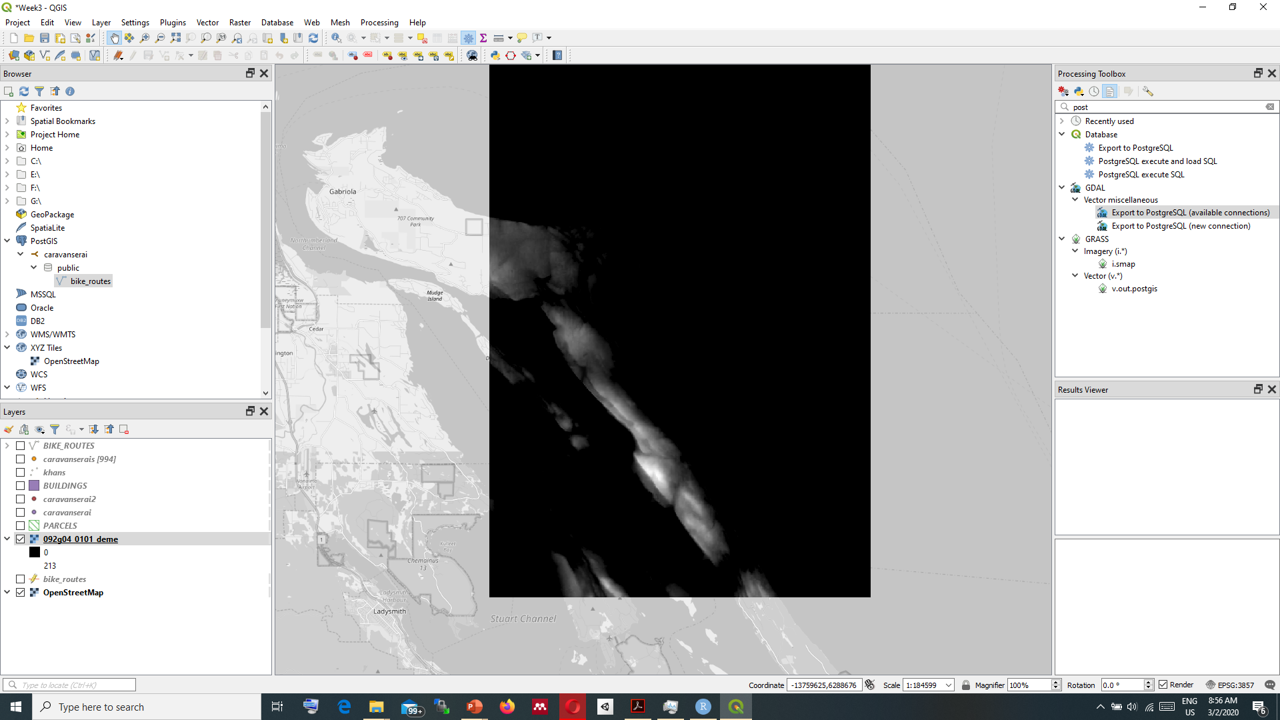
\includegraphics{Images/DEM.png}
\caption{DEM}
\end{figure}

We can add DEM images similar to other raster files.

We can convert raster DEM files to vector contour lines.

\begin{quote}
GDAL\textgreater Raster extraction\textgreater Contour
\end{quote}

\begin{figure}
\centering
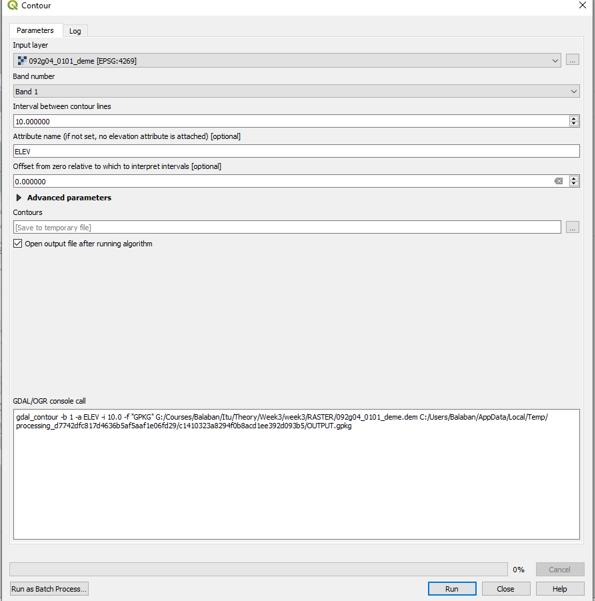
\includegraphics{Images/Contour.png}
\caption{Contour}
\end{figure}

\begin{figure}
\centering
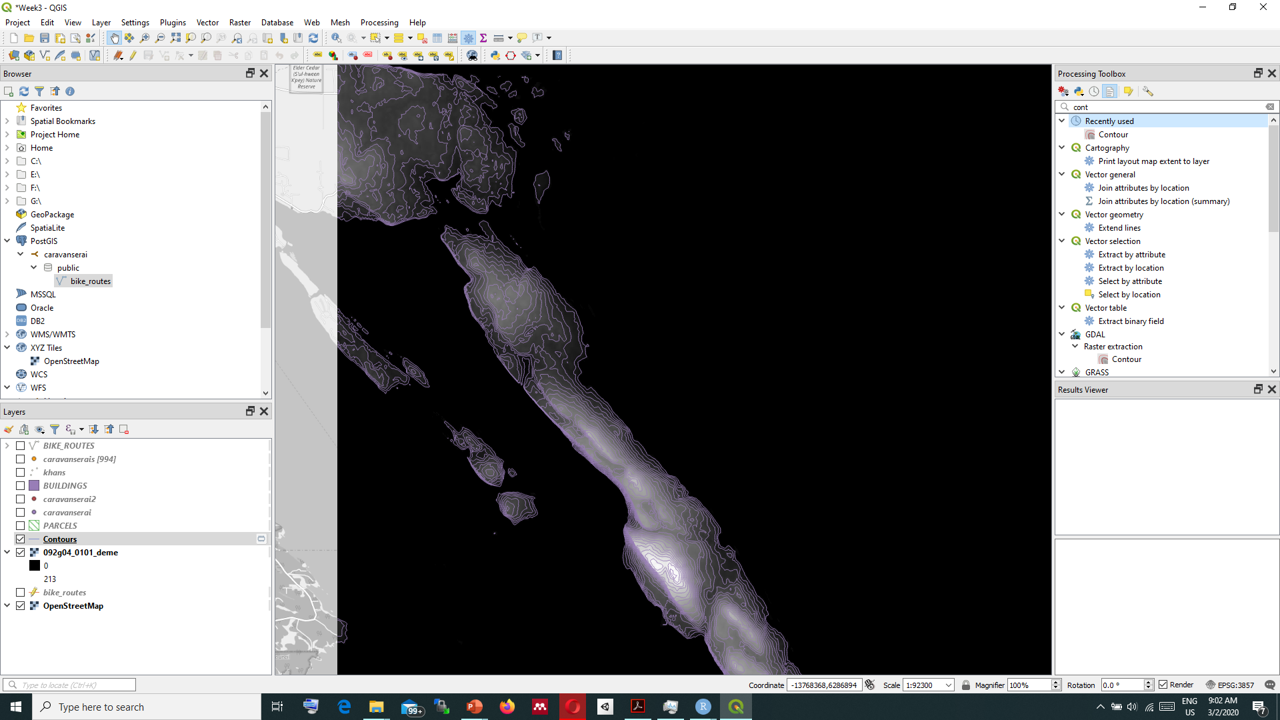
\includegraphics{Images/Contoursfinished.png}
\caption{After extracting the contours}
\end{figure}

\hypertarget{d-maps}{%
\chapter{3D Maps}\label{d-maps}}

We can create 3D maps to visualize the map in 3D. To do this

\begin{quote}
View \textgreater New 3D Map
\end{quote}

\begin{figure}
\centering
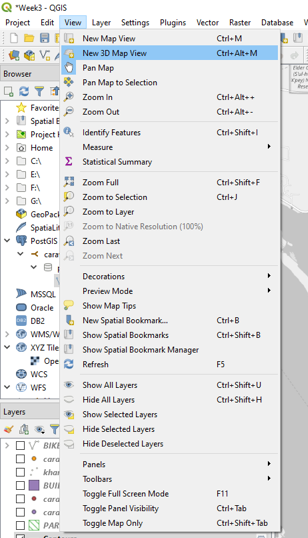
\includegraphics{Images/New3Dmap.png}
\caption{Adding 3D Map}
\end{figure}

That opens up a new window with 3D view. You can adjust, pan, zoom to the map.

\begin{figure}
\centering
\includegraphics{Images/3Dmap.png}
\caption{3D Map Example}
\end{figure}

We can make the vectors from the buildings into 3D objects. For this go to 3D View from layer Properties. Select extrusion and you can set one value for every polygon. Or you can assign a variable by clicking to the icon at the right and setting a variable for extrusion.

\begin{figure}
\centering
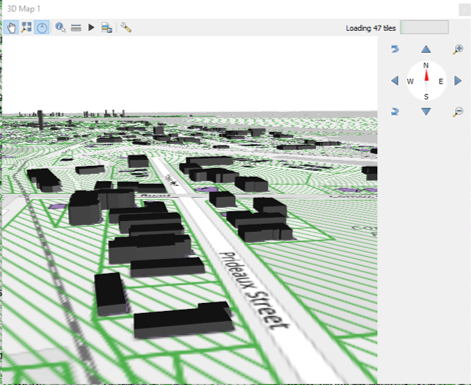
\includegraphics{Images/3Dbuildings.png}
\caption{3D Map Example with 3D polygons}
\end{figure}

\hypertarget{styling-data}{%
\chapter{Styling Data}\label{styling-data}}

QGIS is very flexible in styling data. We can style our layers to visualize the information better.

\hypertarget{points}{%
\section{Points}\label{points}}

\hypertarget{polylines}{%
\section{Polylines}\label{polylines}}

\hypertarget{polygons}{%
\section{Polygons}\label{polygons}}

\hypertarget{raster}{%
\section{Raster}\label{raster}}

\hypertarget{printing-maps}{%
\chapter{Printing Maps}\label{printing-maps}}

\hypertarget{creating-data}{%
\chapter{Creating Data}\label{creating-data}}

\hypertarget{databases}{%
\chapter{Databases}\label{databases}}

\hypertarget{connection-to-postgis-using-ssl}{%
\section{Connection to POSTGIS using SSL}\label{connection-to-postgis-using-ssl}}

QGIS has an ability to connect to various different databases. Geopackage, Oracle Spatial, PostGIS, SpatiaLite.

\begin{figure}
\centering
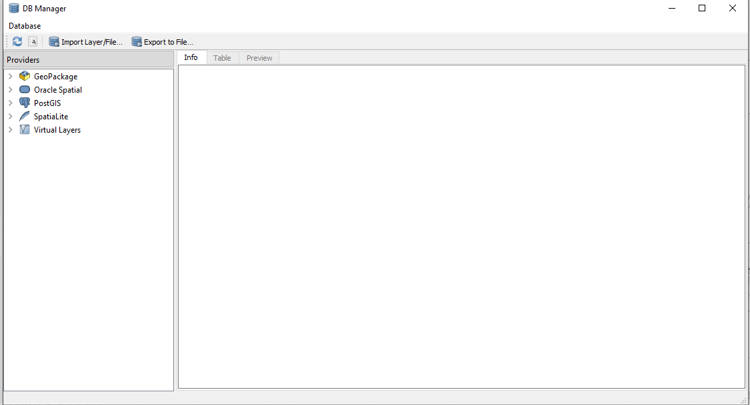
\includegraphics{Images/databases.png}
\caption{Databases that can be connected through QGIS}
\end{figure}

We are going to use PostGIS in our projects.

\begin{quote}
PostGIS is the geographic extension of the database management~system,~PostgreSQL, which allows us to store geographic objects as part of our data tables. A geographic object is a special type~of data that allows us to store a geographic position or a set of them as part of a line or a polygon. Essentially, PostGIS is a powerful tool that enables you to handle complex geographical data and visually explore this data when you use it along with graphical tools, such as QGIS.
\end{quote}

We will be hosting our PostGIS database using Google Cloud.To access it we need to connect using SSL. (However, the eduroam connection in the campus prevents us to use the port 5432 which is the usual postgreSQL port so we need to use out of the ITU network)

To connect you will need to download 3 certificate files. server-ca.pem, client-cert.pem, client-key.pem. Download these files and place them to a folder that is accesible.

From processing toolbox click the right most icon, \textbf{options}.

From the menu select \textbf{Authentication}.

\begin{figure}
\centering
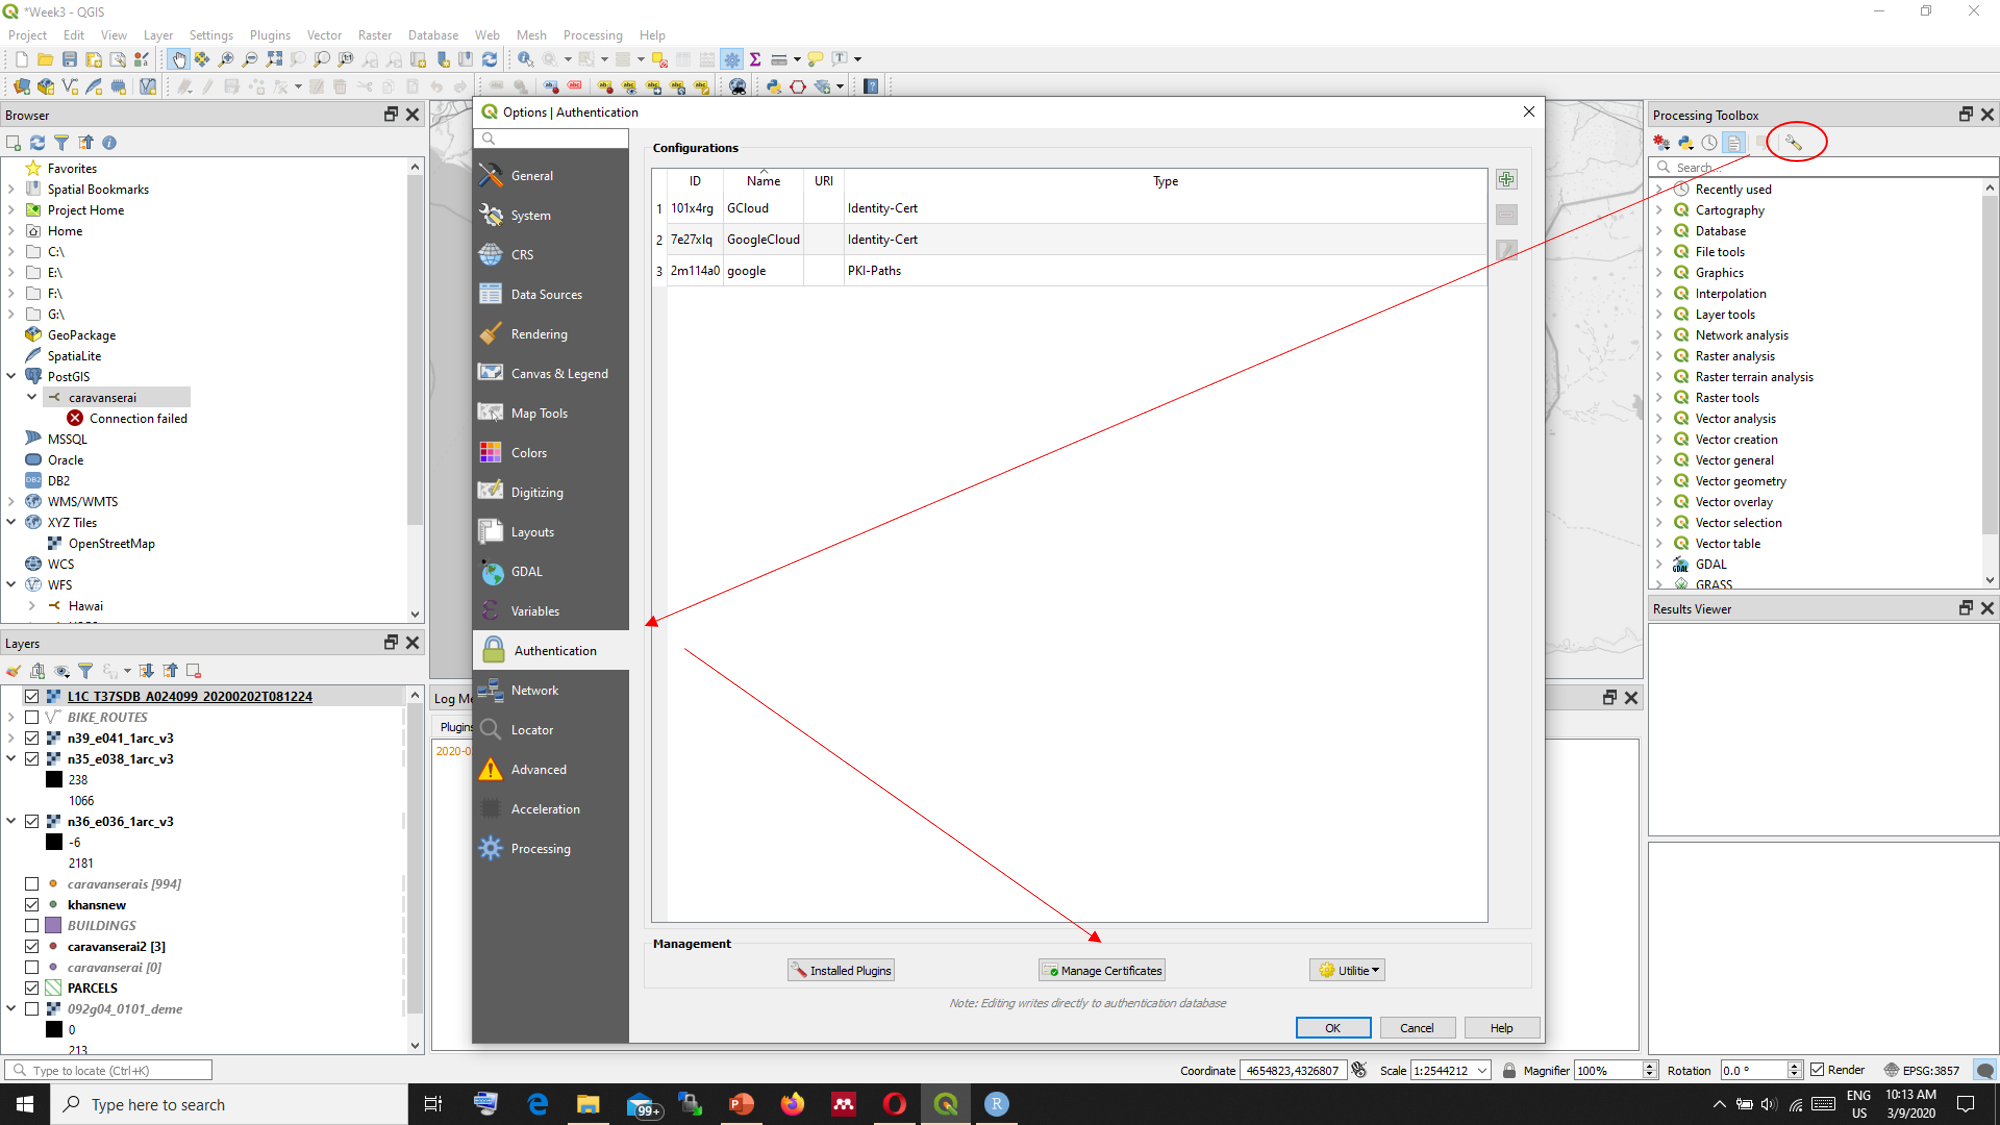
\includegraphics{Images/ManageCertificates.png}
\caption{Manage Certificates}
\end{figure}

And next select \textbf{manage certificates}.

Here from the authorities tab, click + to add Google Cloud certificate.

\begin{figure}
\centering
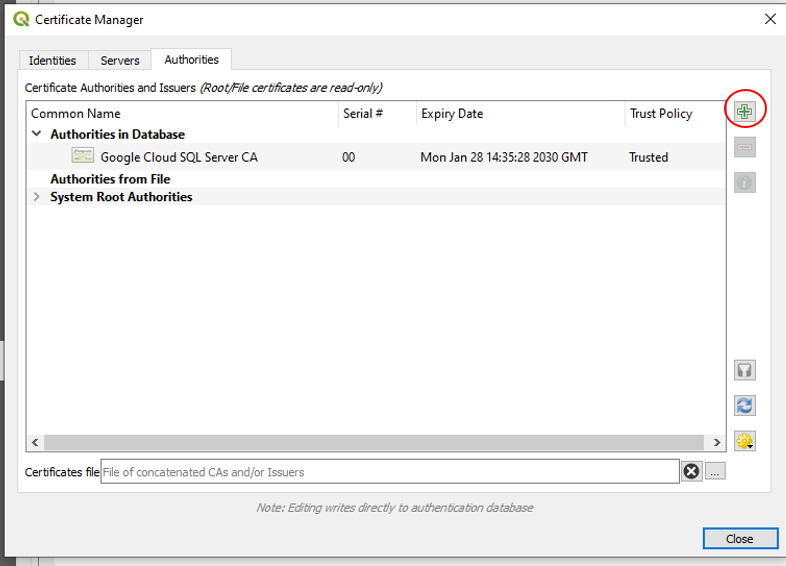
\includegraphics{Images/certificatemanager.png}
\caption{Certificate Manager}
\end{figure}

Here from the import certificate menu, click \ldots{} icon and locate your server-ca.pem file.

\begin{figure}
\centering
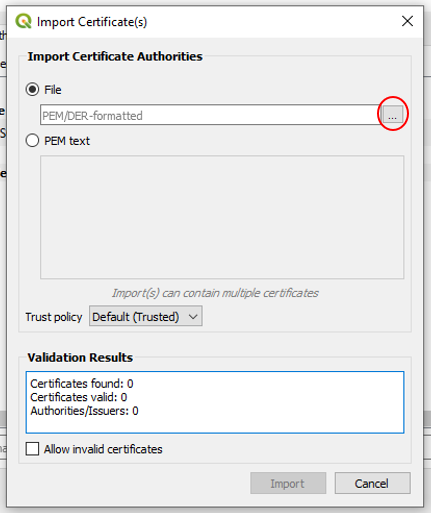
\includegraphics{Images/importcertificate.png}
\caption{Import Certificate}
\end{figure}

Back from the certificate manager screen click to the identities tab and click + icon.

\begin{figure}
\centering
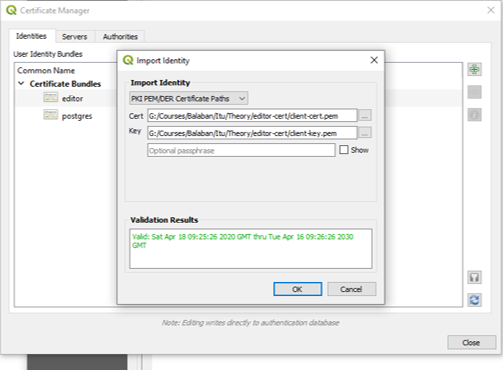
\includegraphics{Images/importIdentity.png}
\caption{Import Identities}
\end{figure}

From the import identity screen, select PKI PEM/DER Certificate Paths. For cert select client-cert.pem and for key select client-key.pem.

Next, close the identity screen and from the Authentication screen click + icon.

\begin{figure}
\centering
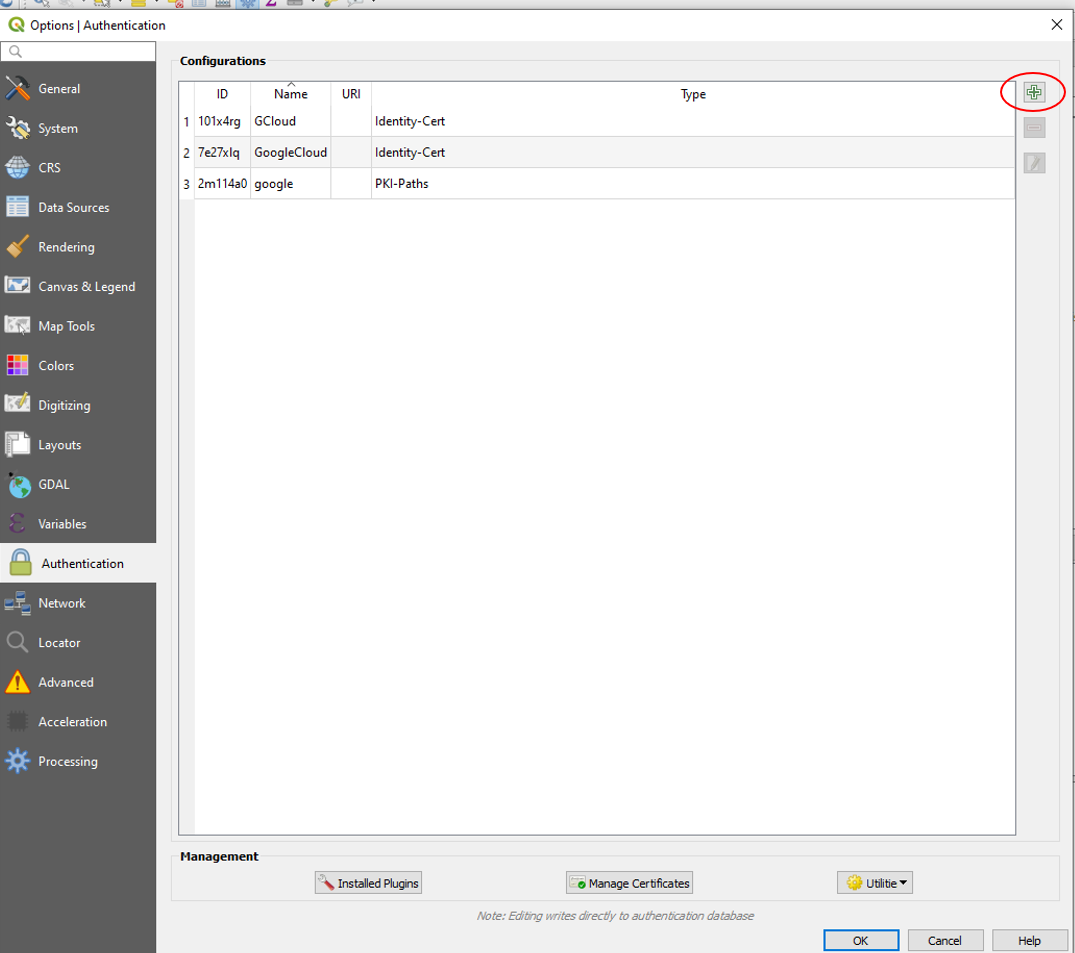
\includegraphics{Images/authentication.png}
\caption{Authentication window}
\end{figure}

From the dialogue box, select PKI stored identity certificate, and select the certificate that you have created (editor). write a name (eg. Google Cloud) and save.

\begin{figure}
\centering
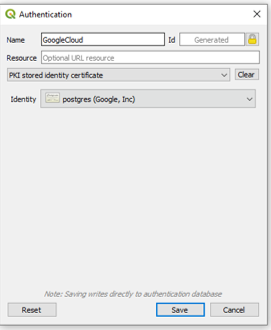
\includegraphics{Images/authentication2.png}
\caption{Authentication Dialogue Box}
\end{figure}

Now close the windows and from the browser panel select PostGIS and right click and select new connection.

\begin{figure}
\centering
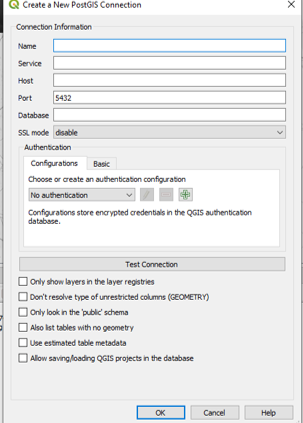
\includegraphics{Images/postgisServer.png}
\caption{PostGIS server settings}
\end{figure}

Here you need to enter information required to setup a connection to our server. Fill out the information as following:

\begin{figure}
\centering
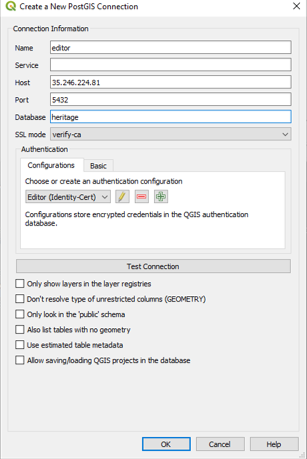
\includegraphics{Images/postGISinfo.png}
\caption{PostGIS information}
\end{figure}

The username and password for our database is \textbf{editor} and \textbf{123post}. After this step we will be connected to the server.

Server connections work similar to the layers. If you have a geospatial data you can import or export to the database.

For this project, we need to have a database of caravanserais as point geometries and we need topography information as vector layer.

\hypertarget{introduction-to-postgis}{%
\section{Introduction to POSTGIS}\label{introduction-to-postgis}}

After connecting to the database, you can see our two tables iran\_han and turk\_han on the left side of the screen.

\begin{figure}
\centering
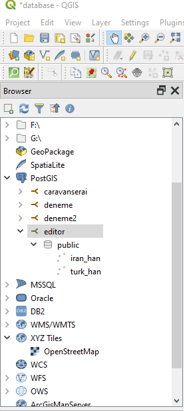
\includegraphics{Images/postgisConnection.png}
\caption{PostGIS Connection}
\end{figure}

POSTGIS database uses SQL Structured Query Language , to create the table turk\_han I used the following SQL query (Showing this for you as a reference you dont need to do this, I already created our tables.)

\begin{verbatim}
CREATE TABLE turk_han  ( id serial, 
common_names character(30),  
alternative_names character(100), 
village character(30), 
district character(30), 
province character(30), 
date character(30), 
reference varchar, 
layer character(10),  
the_geom geometry,    
CONSTRAINT turk_pkey PRIMARY KEY (id)  );
\end{verbatim}

To insert a new feature/han we need to run a sql query. Below you can see an example feature.

\begin{verbatim}
INSERT INTO turk_han (common_names, 
alternative_names, 
village, 
district, 
province, 
date, 
reference, 
layer, 
the_geom) 
VALUES ('Alacahan Kervansarayı', NULL, 'Alacahan', 'Kangal', 'Sivas', '1150-1180', NULL, 'VAR', ST_GeomFromEWKT('SRID=4326;POINT(37.5975095 39.1058708)'));
\end{verbatim}

To update data you need to first find the id of the feature that you want to change. For this you can use SELECT query.

\begin{verbatim}
SELECT * FROM turk_han
WHERE common_name = 'Alacahan Kervansarayı'
\end{verbatim}

For example this query brings all the entries that has common\_name as Alacahan Kervansarayı. For example, to update its location you can use the query below.

\begin{verbatim}
UPDATE turk_han
SET the_geom = ST_GeomFromEWKT('SRID=4326;POINT(37.5975095 39.10587)')
WHERE
    id = 4;
\end{verbatim}

\hypertarget{assignment}{%
\chapter{Assignment}\label{assignment}}

You have been collecting data from the written resources.The primary resources were:

\begin{itemize}
\tightlist
\item
  International database on caravanserais, OWTRAD
\item
  Academic publications, ACUN, ERDMANN, ILTER, CEKUL, etc..
\item
  Websites by travelers, TURKISHHANS
\end{itemize}

You have been using QGIS, Google Earth, Gsheet, Gdrive to structure the data. As our approach is rather Geotemporal, for the next step, you will be using the central database of QGIS.

Next step will to explore the ACCURACY of the data:

\begin{itemize}
\item
  Level 1: REGISTERED HISTORICAL BUILDINGS (TESCILLI BINALAR) by Ministry of Culture and Tourism, State Museums/Sites (Müzeler ve Ören Yerleri), Local Authorities (Belediyeler):

  \begin{itemize}
  \tightlist
  \item
    \url{https://www.kulturportali.gov.tr/}
  \item
    \url{https://muze.gov.tr/muzeler}
  \end{itemize}
\item
  Level 2: Researched Historical Buildings by Local and Academic Authorities.
  ÇEKÜL: \url{https://www.cekulvakfi.org.tr/}
  International Universities
  Local/National Universities
\item
  Level 3: Travelers, Touristic Informations, Locals
\item
  Level 4: Digital Tools and Methods
\end{itemize}

\begin{table}

\caption{\label{tab:unnamed-chunk-2}Assigned Areas}
\centering
\begin{tabular}[t]{r|l|l}
\hline
n & location & name\\
\hline
1 & Bursa - Konya & AYS\\
\hline
2 & Denizli- Alanya- Konya & TAN\\
\hline
3 & Mersin - Aksaray- Konya & NUR\\
\hline
4 & Konya - Aksaray - Nevsehir & BEG\\
\hline
5 & Sakarya - Kayseri- Sivas & SUM\\
\hline
6 & Sinop - Sivas - Malatya & VAR\\
\hline
7 & Urfa - Kayseri & CEM\\
\hline
8 & Mardin - Sivas & FEY-GUL\\
\hline
9 & Igdir - Sivas & SEN\\
\hline
10 &  & SAT\\
\hline
11 &  & NIM\\
\hline
12 &  & SEP\\
\hline
\end{tabular}
\end{table}

\hypertarget{collecting-the-data-creating-the-layer}{%
\section{Collecting the data \& Creating the layer}\label{collecting-the-data-creating-the-layer}}

First step for this assignment is to gather the location info for the caravanserais that you are assigned.

Create a GeoPackage layer.

\begin{quote}
Layer\textgreater Create Layer\textgreater New GeoPackage Layer\ldots{}
\end{quote}

\begin{figure}
\centering
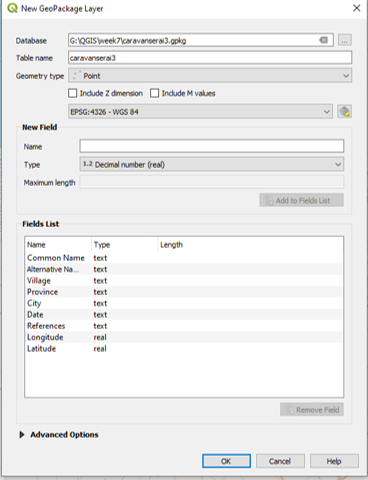
\includegraphics{Images/geopackage.png}
\caption{Create GeoPackage Layer}
\end{figure}

After creating an empty geopackage layer, we are going to create our caravanserais as points.

Right click on the created layer and select \textbf{Open Attribute Table}.

Here you can see our empty table we need to create as many fields as we require. We will at least require Name field as text and Longitude and Latitude as decimal fields. In this table to edit the layer we need to click on the \textbf{Toggle Editing mode} icon. Enter the fields with the collected data.

\begin{figure}
\centering
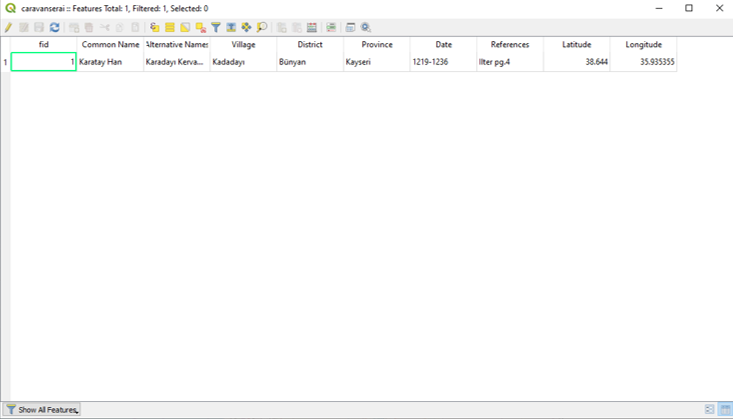
\includegraphics{Images/caravanseraiTable.png}
\caption{Create GeoPackage Layer}
\end{figure}

After creating all the features in our table we need to create the point geometries that is on the coordinates that we entered. For this, we are going to use \textbf{Create points layer from table} from processing toolbox.

\begin{figure}
\centering
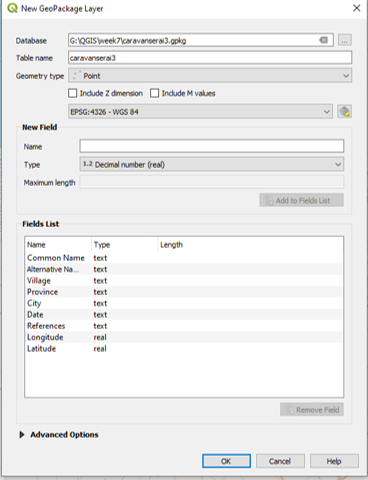
\includegraphics{Images/geopackage.png}
\caption{Create GeoPackage Layer}
\end{figure}

After creating an empty geopackage layer, we are going to create our caravanserais as points.

Right click on the created layer and select \textbf{Open Attribute Table}.

Here you can see our empty table we need to create as many fields as we require. We will at least require Name field as text and Longitude and Latitude as decimal fields. In this table to edit the layer we need to click on the \textbf{Toggle Editing mode} icon. Enter the fields with the collected data.

\begin{figure}
\centering
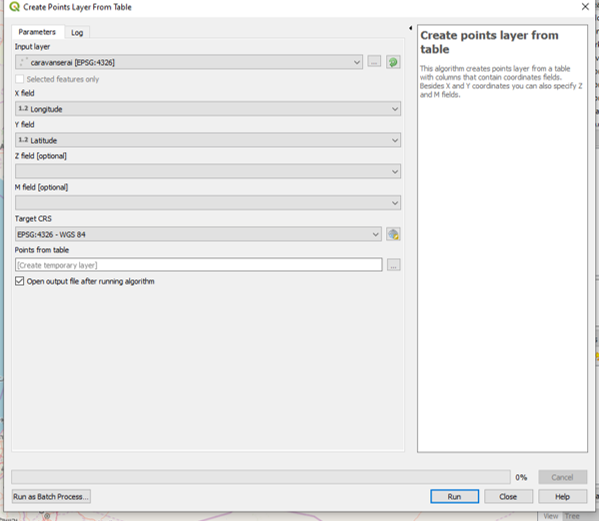
\includegraphics{Images/createpoints.png}
\caption{Create Points Layer from table}
\end{figure}

  \bibliography{book.bib,packages.bib}

\end{document}
